\documentclass[12pt]{article}
\usepackage{graphicx}
\usepackage{a4wide}
\usepackage{url}

\author{C\'edric Pradalier (cedric.pradalier@skybotix.com)}
\title{Bluetooth-based firmware upgrade for the CoaX helicopter}


\begin{document}
\maketitle

\section{Purpose of this document}
This document describes the procedure for upgrading the firmware of the CoaX
helicopter using the bluetooth bootloader. It assumes a global knowledge of
CoaX helicopter and its hardware, as described in \url{http://www.skybotix.com/support/wiki/index.php/Main_Page}.

The bootloader uses a bluetooth protocol emulating a wireless serial link
(RFCOMM). Most of these functions have been heavily tested under Linux. 
Under windows, the support of bluetooth serial device is not extremely
reliable, but the Python GUI has been seen working.

\section{Using the Python GUI}
Note that older CoaX boards (id < 30) have been delivered with a version of the
bootloader firmware that is not compatible with the Python GUI. We strongly
recommend upgrading the bootloader firmware in this case. This is explained in
section~\ref{sec:bootloader-upgrade}.

\subsection{Establishing the bluetooth serial connection under linux}
The first step is to identify the address of the bluetooth device installed on
the CoaX helicopter. The hcitool command can be used (on some systems you may
need to prefix it by sudo, or even be root to use it):
\begin{verbatim}
#>hcitool scan
Scanning ...
	10:00:E8:C0:AC:C8	CoaX_0041
\end{verbatim}
The 6 numbers on the left are the address we are looking for. The rfcomm
command can then be used to establish the connection (again, you may need to be
root to run it):
\begin{verbatim}
#> rfcomm connect 0 10:00:E8:C0:AC:C8
Connected /dev/rfcomm0 to 10:00:E8:C0:AC:C8 on channel 1
Press CTRL-C for hangup

\end{verbatim}
The argument ``0'' of rfcomm is the channel number. This channel will be linked
to a device /dev/rfcomm0 (the zero is the same). The last argument is the
device address.

During the first connection, the bluetooth system will require to enter a
password. For each CoaX board, the password is the 4-digit number corresponding
to the board id. For instance, the board CoaX\_0041 has the string "0041" for
password. See figure \ref{fig:bluetooth-auth-linux} for an example.
\begin{figure}[hb]
\centering
\fbox{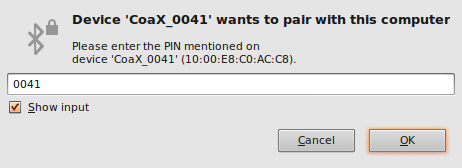
\includegraphics[width=0.7\columnwidth]{bluetooth-auth}}
\caption{Authentification under linux (ubuntu 10.04).}
\label{fig:bluetooth-auth-linux}
\end{figure}

When the connection is not needed anymore, the connection can be closed by
hitting Ctrl-C. 

\subsection{Establishing the bluetooth serial connection under windows}
Using the bluetooth panel should show the coax device. Double clicking on it
will initialise the connection process and require the device password.
For each CoaX board, the password is the 4-digit number corresponding
to the board id. For instance, the board CoaX\_0041 has the string "0041" for
password.

Once the connection is established, Windows has created a COM device. You need
to open the device manager and search the serial port section for a new device.
The name will be COM plus a number, usually greater than 4.

\subsection{Uploading the firmware: principle}
\label{sec:principle}
The next steps will assume that a bluetooth serial connection to the CoaX board
has been established. It has been heavily tested under linux, and has been seen
to work under windows XP.

The principle of the upload process is as follows:
\begin{itemize}
\item The bootloader preload a .hex file containing the firmware to upload.
These files can be obtained from the Skybotix download page, or compiled by
hand using gcc\footnote{Version modified by Microchip for the dsPIC} or the
Microchip development environment under windows.
\item When the CoaX board boots, it sends a character indicating that it is
ready to receive a firmware and waits a second for a proposal. If no
proposal is received during this time, the boards goes on and runs the current
firmware.
\item If a firmware proposal is proposed, the board goes into the upload mode,
and waits for the firmware packets. The PC application starts then to send the
firmware packets, first erasing the existing memory, and then writing the new
firmware. 
\item When the upload is completed, the board reboot itself, and starts the new
firmware. 
\end{itemize}

\subsection{Uploading with the GUI}
Under linux, the GUI can be started by going to the pybootloader directory
(from the CD or a svn checkout), and running the BootloaderGUI.py program.
Depending on your system, this may require to be prefixed by sudo. The gui is
depicted in fig.~\ref{fig:bootloadergui}. 
\begin{figure}[hb!]
\centering
\fbox{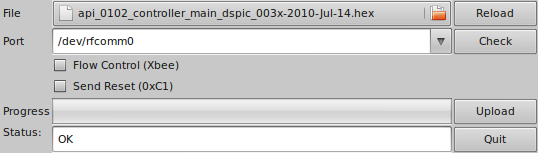
\includegraphics[width=0.7\columnwidth]{bootloadergui}}
\fbox{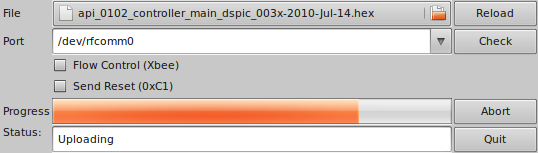
\includegraphics[width=0.7\columnwidth]{bootloadergui2}}
\fbox{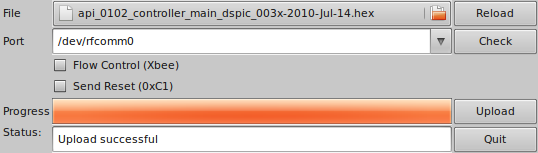
\includegraphics[width=0.7\columnwidth]{bootloadergui3}}
\caption{Multiple steps of the upload gui. Top: configuration before hitting
the upload button. Middle: while uploading. Bottom: uploading completed.}
\label{fig:bootloadergui}
\end{figure}

The GUI is composed of several elements as detailed below:
\begin{itemize}
\item The file drop-box provides a way to select the firmware file. It must be
a .hex file.
\item The port entry should be modified to reflect the port used by the serial
connection (usually /dev/rfcomm0 or COMxx). 
\item Flow Control must be checked when using a Xbee connection instead of the
bluetooth. In this case, the Xbee module is generally visible on /dev/ttyUSB0.
This has not been successfully tested under windows.
\item Send Reset must not be checked on the CoaX board.
\item The Reload button is used to reload a firmware file, for instance after
recompiling it.
\item The Check button will try to open the serial port and report success or
failure. 
\item The Upload button starts the upload process once the file and the port
have been configured. When the upload process starts, it first (re-)read the
.hex file, then open the serial port, and wait for the ready token on the
serial channel. This is triggered by hitting the reset button on the CoaX
board. 
\end{itemize}

The following text output shows some debug message output during the upload
process. The sequence of ``!\_'' indicates that the GUI is waiting for the board
to send the ``ready'' token. Once this is started, the ``X'' symbols correspond
to the packets requesting a memory erase on the dsPIC, whereas the '\#' symbols
correspond to the packets containing the new firmware to write. 
\begin{verbatim}
#> ./BootloaderGUI.py 
File controller\_main\_dspic\_003x-2010-Jul-14.hex selected 
Trying to load u'controller\_main\_dspic\_003x-2010-Jul-14.hex'
%%%%...
Program at address 000000
$$$$...
Created 306 packets, 19584 words to upload (58752 bytes)
Added 39 erase packets
Trying to open /dev/rfcomm0
!_!_!_!_!_!_!_!_!_!_!_!
XXXXXXXXXXXXXXXXXXXXXXXXXXXXXXXXXXXXXXX##############################
#####################################################################
#####################################################################
#####################################################################
#################################
\end{verbatim}

\section{Upgrading the bootloader firmware}
\label{sec:bootloader-upgrade}
The bootloader firmware can be found on the Skybotix download page. It must be
programmed on the main dsPIC using the programmation board and a Microchip
programmer (ICD2 or ICD3). Once the bootloader is written to the dsPIC, then
the procedure described in the previous section must be used to upload a
firmware.

\section{Using coaxuploadbt}
This method only work for linux, for older version of the bootloader firmware
(board id < 30).
The coaxuploadbt executable can be found and compiled in the btbootloader
directory (from the CD or on the SVN repository). To compile it, just run make
in the btbootloader directory. This program depends on the libbluetooth package
(including the development files). 

Running the uploader on the command line is done as follows:
\begin{verbatim}
#>./coaxuploadbt controller-coax002x.hex 41 
coax bluetooth uploader (using libbluetooth) version 2
(c) 2006 - 2009 Olivier Michel, Stephane Magnenat, Cedric Pradalier
Program located at 000200
Upload size: 307 packets 19648 words (58944 bytes)
Added 39 erase packets
Scanning bluetooth:
	10:00:E8:C0:AC:C8 CoaX_0041
Contacting Coax 41
Press enter and then reset on the robot

........................
\end{verbatim}

Note that this method does not require to establish the serial connection
beforehand. It will fail on CoaX boards equipped with the newer bootloader
firmware due to a significant change in the bootloader protocol. 

\end{document}

